%%%%%%%%%%%%%%%%%%%%%%%%%%%%%%%%%%%%%%%%%
% Awesome Resume/CV
% XeLaTeX Template
% Version 1.1 (9/1/2016)
%
% This template has been downloaded from:
% http://www.LaTeXTemplates.com
%
% Original author:
% Claud D. Park (posquit0.bj@gmail.com) with modifications by
% Vel (vel@latextemplates.com)
%
% License:
% CC BY-NC-SA 3.0 (http://creativecommons.org/licenses/by-nc-sa/3.0/)
%
% Important note:
% This template must be compiled with XeLaTeX, the below lines will ensure this
%!TEX TS-program = xelatex
%!TEX encoding = UTF-8 Unicode
%
%%%%%%%%%%%%%%%%%%%%%%%%%%%%%%%%%%%%%%%%%

%----------------------------------------------------------------------------------------
%   PACKAGES AND OTHER DOCUMENT CONFIGURATIONS
%----------------------------------------------------------------------------------------

\documentclass[12pt, a4paper]{awesome-cv} % A4 paper size by default, use 'letterpaper' for US letter

\geometry{left=2cm, top=1.5cm, right=2cm, bottom=2cm, footskip=.5cm} % Configure page margins with geometry

\fontdir[fonts/] % Specify the location of the included fonts

% Color for highlights
\colorlet{awesome}{awesome-concrete} % Default colors include: awesome-emerald, awesome-skyblue, awesome-red, awesome-pink, awesome-orange, awesome-nephritis, awesome-concrete, awesome-darknight
%\definecolor{awesome}{HTML}{CA63A8} % Uncomment if you would like to specify your own color

% Colors for text - uncomment and modify
%\definecolor{darktext}{HTML}{414141}
%\definecolor{text}{HTML}{414141}
%\definecolor{graytext}{HTML}{414141}
%\definecolor{lighttext}{HTML}{414141}

\renewcommand{\acvHeaderSocialSep}{\quad\textbar\quad} % If you would like to change the social information separator from a pipe (|) to something else

% ----------------------------------------------------------------------------------------
%   PERSONAL INFORMATION
%   Comment any of the lines below if they are not required
%----------------------------------------------------------------------------------------

\name{Bharat}{Singh}
% \address{Centre for Converging Technologies, University of Rajasthan,
% Jaipur, Rajasthan}
\address{University of Rajasthan Jaipur}
\mobile{(+91) 9636225266}

\email{006.rajpurohit@gmail.com}
\homepage{https://bharatpurohit97.github.io/}
\github{https://github.com/bharatpurohit97}
%\linkedin{https://www.linkedin.com/in/bharat-purohit-963683109/}
%\skype{skypeid}
%\stackoverflow{SOid}{SOname}
%\twitter{@twit}

\position{B.Tech - M.Tech Dual Degree{\enskip\cdotp\enskip}Information and Communication Technology and Cognitive Neuroscience (Minor)} % Your expertise/fields
%\quote{``Make the change that you want to see in the world."} % A
%quote or statement

\makecvfooter{\today}{Bharat Singh~~~·~~~Resume}{\thepage}

%----------------------------------------------------------------------------------------

% \usepackage{tikz}

\begin{document}

\makecvheader % Print the header

% \tikz[remember picture,overlay]
%   \node[anchor=north east,inner sep=0pt] at (current page.north east)
%     {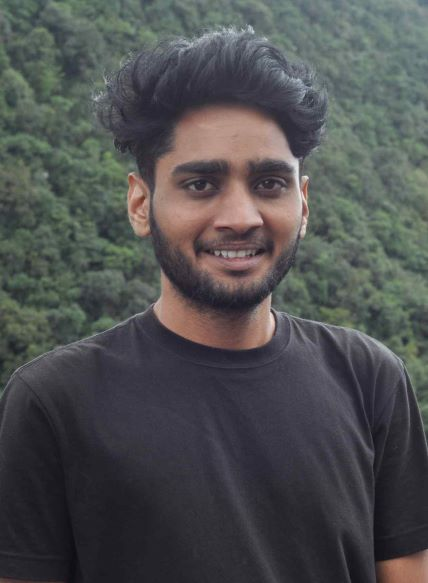
\includegraphics[height=4cm]{me}};

    % ----------------------------------------------------------------------------------------
%   CV/RESUME CONTENT
%   Each section is imported separately, open each file in turn to modify content
%----------------------------------------------------------------------------------------

%----------------------------------------------------------------------------------------
%   SECTION TITLE
%----------------------------------------------------------------------------------------

\cvsection{Education}

%----------------------------------------------------------------------------------------
%   SECTION CONTENT
%----------------------------------------------------------------------------------------

\begin{cventries}

%------------------------------------------------

\cventry
{B.Tech - M.Tech Dual Degree, Information and Communication Technology and Minor in Cognitive Neuroscience} % Degree
{Centre for Converging Technologies, University of Rajasthan} % Institution
{Jaipur, India} % Location
{2015 - 2020} % Date(s)
{% Description(s) bullet points
\begin{cvitems}
\item {Rank in Top 3. Cumulative Performance Index /
    \textbf{CGPA: 4.6/6.0}}
\end{cvitems}
}

\end{cventries}

%%% Local Variables:
%%% mode: xelatex
%%% TeX-master: "../resume_twopage"
%%% End:

% ----------------------------------------------------------------------------------------
% SECTION TITLE
% ----------------------------------------------------------------------------------------

\vspace{-0.2cm}
\cvsection{Work Experience}

% ----------------------------------------------------------------------------------------
% SECTION CONTENT
% ----------------------------------------------------------------------------------------

\begin{cventries}

  % ------------------------------------------------

  \cventry
  {Research Intern, BTISnet Jaipur}
  {Bioinformatics Infrastructure Facility, Department of Biotechnology (DBT)}
  {Jaipur, Rajasthan}
  {July. 2018 - Present}
  {
    \begin{cvitems}
    \item {Worked on Google BigQuery, AWS services, Galaxy to Annotate, Align and Querying Genomic Databases, features requested by industry in Bio-informatics.}
    \item {Created a web enabled tool for finding unique DNA fragment. project includes database and phylogeny tree creation. it involves use of graph data structure, MongoDB, Searching, allignments, kmer manipulations and bioinformatics for client-servers }
    % \item {Designed a method for allowing key rotations in a multi-master system with a shared database.}
    \item {Designed Algorithms for Extraction, Preprocessing, Sequencing, Searching of Genomic Database and Networking for phylogeny using Python, shell scripting. Used Machine learning and statistical inference for data analysis, classification and prediction in Genomic database}
    \end{cvitems}
  }


  \cventry
  {Full Stack Developer, under Prof. Abhilasha Dangi}
  {CCT Department, University of Rajasthan}
  {Jaipur, India}
  {Feb. 2017 - May. 2017}
  {
    \begin{cvitems}
    \item Worked on a scalable microservice based web application with an extensive technology stack.
    \item Designed and developed critical backend features while
      ensuring type-safety.
    \item Developed and deployed the complete functionality in institution
    \item Adjudged as one of the best project, while being a freshman.
    \end{cvitems}
  }

  % ------------------------------------------------
\end{cventries}

%%% Local Variables:
%%% mode: xelatex
%%% TeX-master: "../resume_twopage"
%%% End:

% ----------------------------------------------------------------------------------------
% SECTION TITLE
% ----------------------------------------------------------------------------------------
\cvsection{Projects}

% ----------------------------------------------------------------------------------------
% SECTION CONTENT
% ----------------------------------------------------------------------------------------

\begin{cventries}

  % ------------------------------------------------
  \cventry
  {Research Project, Prof. Sumita Kachhwaha}
  {\href{https://github.com/DBT-BIF/Biosensor-Python}{\entrytitlestyle{Biosensor-Python}}
    {}}
  {DBT-BIF Jaipur}
  {July. 2018 - Sept. 2018}
  {
    \begin{cvitems}
    \item Created a web enabled tool for finding unique DNA fragment that also draw phylogeny
     of life.
    \item Designed a module in python for Extraction, Parsing, Pre-processing, Sequencing, Searching of Genomic Database and Networking for phylogeny of life.
    \item Used Machine learning and statistical inference for classification and prediction in Genomic database
    \end{cvitems}
  }
  \cventry
  {Course Project, Prof. Abhilasha Dangi}
  {\entrytitlestyle{Senior Students Placement Cell}}
  {University of Rajasthan, Jaipur}
  {Feb. 2017 - May. 2017}
  {
    \begin{cvitems}
      \item Conceptualized new web 2.0 based IT services such as Interest Group Discussion Forums,
       Senior alumni Information and contacts, Campus Wiki, Project Database
      \item Allow easier collaboration, better information organization and formalizing
       undocumented technical.
      \item Designed intuitive user interfaces and work-flows for these services and
       customization then finally deploy these services in the institute
    \end{cvitems}
  }
    
  \cventry
  {Research Project, Team of 2 members}
  {\entrytitlestyle{Thought Reading Device: Predicting Text by EEG signals (BCI)}}
  {IIT Guwahati}
  {Nov. 2016 - March. 2017}
  {
    \begin{cvitems}
      \item Designed Computational model to infer psychological state of human brain with one colleague.
      \item used BrainIAK software that allows for decoding digital brain data to reveal
      how neural activity give rises to learning, memory and other cognitive function.
      \item Used viterbi force alignment and hidden markov model for mapping phone sequences to word. 
    \end{cvitems}
  }

%  \cventry
%  {Individual Project, Dr. Rakesh Sharma}
%  {\entrytitlestyle{PageMatrix : Co-founder}}
%  {Jaipur}
%  {May. 2018 - Aug. 2018}
%  {
%    \begin{cvitems}
%      \item Designed and Developed a SEO Tool for Page-ranking, Links and Emails 
%        Extraction and Keyword prediction for websites with team of three members.
%      \item Build Python scripts and used Django, Shell scripting to set up Frontend, Backend
%        and Sqlite3 for database.
%      \item Deployed on web for 3 months, with 1800+ users and 45 matches.
%    \end{cvitems}
%  }

  \cventry
  {Leader, Team SudoHack Project}
  {\href{https://github.com/LNMHacks/LNMHacks-3.0-Submission/sudo hack}{\entrytitlestyle{Pneumonia Detection: Deep learning}}}
  {CCT Jaipur}
  {Sep. 2018 - Nov. 2018}
  {
    \begin{cvitems}
      \item Build an algorithm that shows good confidence interval in detecting pneumonia
        and Automatically locate lung opacities on chest radiographs and medical images. 
      \item Used TensorFow, CNN model: DenseNet169 for transfer learning,
        and predict lung opacity by loading models.
      \item Finished in top 10 teams from all over India at LNMHacks 3.0.
    \end{cvitems}
  }
 


  % ------------------------------------------------
\end{cventries}

%%% Local Variables:
%%% mode: xelatex
%%% TeX-master: "../resume_twopage.tex"
%%% End:

% ----------------------------------------------------------------------------------------
% SECTION TITLE
% ----------------------------------------------------------------------------------------

\vspace{-0.3cm}
\cvsection{Conferences/Workshops \& Certificates}

% ----------------------------------------------------------------------------------------
% INTERNATIONAL SUBSECTION
% ----------------------------------------------------------------------------------------

% ------------------------------------------------

\begin{cvhonors}

  % ------------------------------------------------

  \cvhonor
  {National Symposium on Cognitive Science} % Award
  {Poster:"Thought Reading Device"} % Event
  {IIT Guwahati} % Location
  {2017} % Date(s)

  % ------------------------------------------------
  \cvhonor
  {High Performance Computing}
  {Techfest IIT Bombay}
  {IIT Bombay}
  {2016}
  \cvhonor
  {Annual Conference of Cognitive Science} % Award
  {Participant}
  {IIT Guwahati} % Location
  {2018} % Date(s)
  % ------------------------------------------------
  \cvhonor
  {Young Statisticians Meet:Data Science in action} % Award
  {Attending} % Event  
  {ISI Kolkata} % Location
  {2019} % Date(s)

  \cvhonor
  {Microsoft Professional Programme: Data science}
  {EdX Certificate}
  {Jaipur}
  {2018}

  \cvhonor
  {Introduction to Machine Learning}
  {NPTEL Certificate}
  {Jaipur}
  {2018}



  % ------------------------------------------------

\end{cvhonors}

%%% Local Variables:
%%% mode: latex
%%% TeX-master: "../resume_twopage.tex"
%%% End:

% ----------------------------------------------------------------------------------------
% SECTION TITLE
% ----------------------------------------------------------------------------------------
\vspace{-0.3cm}
\cvsection{Extracurricular Activity}

% ----------------------------------------------------------------------------------------
% SECTION CONTENT
% ----------------------------------------------------------------------------------------

\begin{cventries}

  \extraentry
  {Centre for Converging Technology, DBT-BIF, Jaipur}
  {Coordinator}
  {Jaipur}
  {2018-19}
  {
    \begin{cvitems}
    \item Lead Organizer of 2 days workshop on \underline{Basics of Bio-Informatics} 
    \item Lead Organized of \href{https://drive.google.com/file/d/1PDJYCQRCsk0e_HojYzUzvAWycQPXnXpg/view?usp=sharing}{\underline{Cloud Computing Seminar}}
    \item Organizer and volunteer of cultural event of Department \underline{JALSA 2K17}
    \end{cvitems}
  }



  \extraentry{}
  {Hackathon Finalist, Winners}
  {Jaipur}
  {March 2018, Oct. 2018}
  {
    \begin{cvitems}
    \item Rajasthan IT Day- eduHack 4.0 - Finalist
    \item LNMHacks 3.0 LNMIIT, Jaipur - Finalist
    \item MLH Local Hack Day, Jaipur - Winners
    \end{cvitems}
  }

  \extraentry
  {\underline{Member}}
  {Cognitive Science Association of India}
  {India}
  {Sept. 2018-Present}
  {}

  \vspace{-0.3cm}


\end{cventries}

%%% Local Variables:
%%% mode: xelatex
%%% TeX-master: "../resume_twopage"
%%% End:

% ----------------------------------------------------------------------------------------
%   SECTION TITLE
% ----------------------------------------------------------------------------------------

\vspace{-0.3cm}
\cvsection{Skills}

% ----------------------------------------------------------------------------------------
%   SECTION CONTENT
% ----------------------------------------------------------------------------------------

\begin{cvskills}

  % ------------------------------------------------

  \cvskill
  {Programming}
  {C/C++, Python, Haskell, MySQL, PHP, Matlab, R}

  % ------------------------------------------------

  \cvskill
  {Web}
  {Django, Flask, Apache Server, CSS, JavaScript }

  % ------------------------------------------------

  \cvskill
  {Utilities}
  {Linux shell utilities, Git, Google Cloud,
    Galaxy, Azure ML Studio, Biopython, \LaTeX}

  % ------------------------------------------------

\end{cvskills}

%%% Local Variables:
%%% mode: latex
%%% TeX-master: "../resume_twopage"
%%% End:

% ----------------------------------------------------------------------------------------
% SECTION TITLE
% ----------------------------------------------------------------------------------------

\vspace{-0.3cm}
\cvsection{Relevant Coursework}

{\fontsize{11pt}{1em}\bodyfontlight\upshape\color{text}
\begin{tabular*}{\textwidth}{L{0.4cm} L{\textwidth/3 - 1cm} L{0.4cm}
  L{\textwidth/3 - 1cm} L{0.4cm} L{\textwidth/3 - 1cm}}
  A$*$ & Machine learning & A$*$ & Artificial Intelligence & A$*$ & Functional Programming \\
  A$*$ & Computer Organization & A$*$ & Computer Network & A$*$ &
    Data Structures and Algos \\
  A$*$ & DBMS & A$*$ & Quantum Computing & A &
    Computational Neuroscience\\
  A & TCP - IP  & A & Dynamical system for Neuroscience \\
\end{tabular*}
\fontsize{11pt}{1em}\footerfont\upshape\color{text}
\begin{tabular*}{\textwidth}{L{8.4cm} L{3cm} L{3.5cm}}
  \entrylocationstyle{A$*$: Grade for exceptional performance} & \entrylocationstyle{A: grade} & \\
\end{tabular*}
\vspace{-6mm}
}

% ----------------------------------------------------------------------------------------
% SECTION CONTENT
% ----------------------------------------------------------------------------------------

%%% mode: xelatex
%%% End:

%%% Local Variables:
%%% mode: latex
%%% TeX-master: "../resume_twopage"
%%% End:

\vspace{-0.2cm}

\cvsection{Miscellaneous}

{\fontsize{11pt}{1em}\bodyfontlight\upshape\color{text}
\begin{itemize}
  \itemsep-0.3em
  \item Blog about Machine learning, Data science and some Programing topics at \href{https://bharatpurohit97.github.io}{bharatpurohit97.github.io}
  \item Contribute to open source projects like Coala,Python,GA4GH on Github.
  \item Administered a cloud in CCT DEPT., deploying and managing services for the campus community.
\end{itemize}
}

%%% Local Variables:
%%% TeX-master: "../resume_twopage"
%%% TeX-engine: xetex
%%% End:


%----------------------------------------------------------------------------------------

\end{document}
%%% Local Variables:
%%% mode: latex
%%% TeX-master: t
%%% TeX-engine: xetex
%%% End:
